\documentclass[twoside]{book}

% Packages required by doxygen
\usepackage{calc}
\usepackage{doxygen}
\usepackage{graphicx}
\usepackage[utf8]{inputenc}
\usepackage{makeidx}
\usepackage{multicol}
\usepackage{multirow}
\usepackage{textcomp}
\usepackage[table]{xcolor}

% NLS support packages
\usepackage[spanish]{babel}
% Font selection
\usepackage[T1]{fontenc}
\usepackage{mathptmx}
\usepackage[scaled=.90]{helvet}
\usepackage{courier}
\usepackage{amssymb}
\usepackage{sectsty}
\renewcommand{\familydefault}{\sfdefault}
\allsectionsfont{%
  \fontseries{bc}\selectfont%
  \color{darkgray}%
}
\renewcommand{\DoxyLabelFont}{%
  \fontseries{bc}\selectfont%
  \color{darkgray}%
}

% Page & text layout
\usepackage{geometry}
\geometry{%
  a4paper,%
  top=2.5cm,%
  bottom=2.5cm,%
  left=2.5cm,%
  right=2.5cm%
}
\tolerance=750
\hfuzz=15pt
\hbadness=750
\setlength{\emergencystretch}{15pt}
\setlength{\parindent}{0cm}
\setlength{\parskip}{0.2cm}
\makeatletter
\renewcommand{\paragraph}{%
  \@startsection{paragraph}{4}{0ex}{-1.0ex}{1.0ex}{%
    \normalfont\normalsize\bfseries\SS@parafont%
  }%
}
\renewcommand{\subparagraph}{%
  \@startsection{subparagraph}{5}{0ex}{-1.0ex}{1.0ex}{%
    \normalfont\normalsize\bfseries\SS@subparafont%
  }%
}
\makeatother

% Headers & footers
\usepackage{fancyhdr}
\pagestyle{fancyplain}
\fancyhead[LE]{\fancyplain{}{\bfseries\thepage}}
\fancyhead[CE]{\fancyplain{}{}}
\fancyhead[RE]{\fancyplain{}{\bfseries\leftmark}}
\fancyhead[LO]{\fancyplain{}{\bfseries\rightmark}}
\fancyhead[CO]{\fancyplain{}{}}
\fancyhead[RO]{\fancyplain{}{\bfseries\thepage}}
\fancyfoot[LE]{\fancyplain{}{}}
\fancyfoot[CE]{\fancyplain{}{}}
\fancyfoot[RE]{\fancyplain{}{\bfseries\scriptsize Generado el Miércoles, 16 de Abril de 2014 09\-:08\-:56 para E\-S\-E por Doxygen }}
\fancyfoot[LO]{\fancyplain{}{\bfseries\scriptsize Generado el Miércoles, 16 de Abril de 2014 09\-:08\-:56 para E\-S\-E por Doxygen }}
\fancyfoot[CO]{\fancyplain{}{}}
\fancyfoot[RO]{\fancyplain{}{}}
\renewcommand{\footrulewidth}{0.4pt}
\renewcommand{\chaptermark}[1]{%
  \markboth{#1}{}%
}
\renewcommand{\sectionmark}[1]{%
  \markright{\thesection\ #1}%
}

% Indices & bibliography
\usepackage{natbib}
\usepackage[titles]{tocloft}
\setcounter{tocdepth}{3}
\setcounter{secnumdepth}{5}
\makeindex

% Hyperlinks (required, but should be loaded last)
\usepackage{ifpdf}
\ifpdf
  \usepackage[pdftex,pagebackref=true]{hyperref}
\else
  \usepackage[ps2pdf,pagebackref=true]{hyperref}
\fi
\hypersetup{%
  colorlinks=true,%
  linkcolor=blue,%
  citecolor=blue,%
  unicode%
}

% Custom commands
\newcommand{\clearemptydoublepage}{%
  \newpage{\pagestyle{empty}\cleardoublepage}%
}


%===== C O N T E N T S =====

\begin{document}

% Titlepage & ToC
\hypersetup{pageanchor=false}
\pagenumbering{roman}
\begin{titlepage}
\vspace*{7cm}
\begin{center}%
{\Large E\-S\-E }\\
\vspace*{1cm}
{\large Generado por Doxygen 1.8.6}\\
\vspace*{0.5cm}
{\small Miércoles, 16 de Abril de 2014 09:08:56}\\
\end{center}
\end{titlepage}
\clearemptydoublepage
\tableofcontents
\clearemptydoublepage
\pagenumbering{arabic}
\hypersetup{pageanchor=true}

%--- Begin generated contents ---
\chapter{Indice jerárquico}
\section{Class Hierarchy}
This inheritance list is sorted roughly, but not completely, alphabetically\+:\begin{DoxyCompactList}
\item \contentsline{section}{zt\+:\+:Animatable}{\pageref{classzt_1_1_animatable}}{}
\begin{DoxyCompactList}
\item \contentsline{section}{zt\+:\+:Animatable\+Container}{\pageref{classzt_1_1_animatable_container}}{}
\item \contentsline{section}{zt\+:\+:Scene}{\pageref{classzt_1_1_scene}}{}
\end{DoxyCompactList}
\item \contentsline{section}{zt\+:\+:Application}{\pageref{classzt_1_1_application}}{}
\item \contentsline{section}{zt\+:\+:Argument}{\pageref{classzt_1_1_argument}}{}
\item \contentsline{section}{zt\+:\+:Arguments}{\pageref{classzt_1_1_arguments}}{}
\item \contentsline{section}{zt\+:\+:Auto\+Lang}{\pageref{classzt_1_1_auto_lang}}{}
\item Clock\begin{DoxyCompactList}
\item \contentsline{section}{zt\+:\+:Clock}{\pageref{classzt_1_1_clock}}{}
\begin{DoxyCompactList}
\item \contentsline{section}{zt\+:\+:Nestable\+Clock}{\pageref{classzt_1_1_nestable_clock}}{}
\end{DoxyCompactList}
\end{DoxyCompactList}
\item \contentsline{section}{zt\+:\+:Discovered\+Node$<$ Node\+Type $>$}{\pageref{classzt_1_1_discovered_node}}{}
\item Drawable\begin{DoxyCompactList}
\item \contentsline{section}{zt\+:\+:Render\+Layer}{\pageref{classzt_1_1_render_layer}}{}
\item \contentsline{section}{zt\+:\+:Tilemap\+Layer$<$ T $>$}{\pageref{classzt_1_1_tilemap_layer}}{}
\item \contentsline{section}{zt\+:\+:Tilemap\+Renderer$<$ T $>$}{\pageref{classzt_1_1_tilemap_renderer}}{}
\end{DoxyCompactList}
\item exception\begin{DoxyCompactList}
\item \contentsline{section}{zt\+:\+:File\+Not\+Found\+Exception}{\pageref{classzt_1_1_file_not_found_exception}}{}
\item \contentsline{section}{zt\+:\+:Resource\+Not\+Found\+Exception}{\pageref{classzt_1_1_resource_not_found_exception}}{}
\end{DoxyCompactList}
\item \contentsline{section}{zt\+:\+:I\+Mesh$<$ Node\+Type $>$}{\pageref{classzt_1_1_i_mesh}}{}
\item \contentsline{section}{zt\+:\+:I\+Node}{\pageref{classzt_1_1_i_node}}{}
\item \contentsline{section}{zt\+:\+:tiled\+:\+:Layer}{\pageref{classzt_1_1tiled_1_1_layer}}{}
\item \contentsline{section}{zt\+:\+:Loading\+Target}{\pageref{classzt_1_1_loading_target}}{}
\begin{DoxyCompactList}
\item \contentsline{section}{zt\+:\+:Resource\+Manager$<$ sf\+:\+:Font $>$}{\pageref{classzt_1_1_resource_manager}}{}
\begin{DoxyCompactList}
\item \contentsline{section}{zt\+:\+:Font\+Manager}{\pageref{classzt_1_1_font_manager}}{}
\end{DoxyCompactList}
\item \contentsline{section}{zt\+:\+:Resource\+Manager$<$ sf\+:\+:Sound\+Buffer $>$}{\pageref{classzt_1_1_resource_manager}}{}
\begin{DoxyCompactList}
\item \contentsline{section}{zt\+:\+:Sound\+Buffer\+Manager}{\pageref{classzt_1_1_sound_buffer_manager}}{}
\end{DoxyCompactList}
\item \contentsline{section}{zt\+:\+:Resource\+Manager$<$ sf\+:\+:Texture $>$}{\pageref{classzt_1_1_resource_manager}}{}
\begin{DoxyCompactList}
\item \contentsline{section}{zt\+:\+:Texture\+Manager}{\pageref{classzt_1_1_texture_manager}}{}
\end{DoxyCompactList}
\item \contentsline{section}{zt\+:\+:Resource\+Manager$<$ X $>$}{\pageref{classzt_1_1_resource_manager}}{}
\end{DoxyCompactList}
\item \contentsline{section}{zt\+:\+:Log}{\pageref{classzt_1_1_log}}{}
\begin{DoxyCompactList}
\item \contentsline{section}{zt\+:\+:Console\+Log}{\pageref{classzt_1_1_console_log}}{}
\item \contentsline{section}{zt\+:\+:File\+Log}{\pageref{classzt_1_1_file_log}}{}
\end{DoxyCompactList}
\item \contentsline{section}{zt\+:\+:tiled\+:\+:Map}{\pageref{classzt_1_1tiled_1_1_map}}{}
\item \contentsline{section}{zt\+:\+:tiled\+:\+:Object}{\pageref{classzt_1_1tiled_1_1_object}}{}
\item \contentsline{section}{zt\+:\+:tiled\+:\+:Object\+Layer}{\pageref{classzt_1_1tiled_1_1_object_layer}}{}
\item \contentsline{section}{zt\+:\+:Package}{\pageref{classzt_1_1_package}}{}
\item \contentsline{section}{zt\+:\+:Package\+File\+Info}{\pageref{classzt_1_1_package_file_info}}{}
\item \contentsline{section}{zt\+:\+:Pathfinding$<$ Node\+Type $>$}{\pageref{classzt_1_1_pathfinding}}{}
\item \contentsline{section}{zt\+:\+:Resource\+Provider}{\pageref{classzt_1_1_resource_provider}}{}
\item \contentsline{section}{zt\+:\+:Scene\+Manager}{\pageref{classzt_1_1_scene_manager}}{}
\item \contentsline{section}{zt\+:\+:Screen\+Dimensions}{\pageref{classzt_1_1_screen_dimensions}}{}
\item \contentsline{section}{zt\+:\+:Singleton$<$ T $>$}{\pageref{classzt_1_1_singleton}}{}
\item \contentsline{section}{zt\+:\+:Task}{\pageref{classzt_1_1_task}}{}
\item \contentsline{section}{zt\+:\+:Task\+Pool}{\pageref{classzt_1_1_task_pool}}{}
\item Text\begin{DoxyCompactList}
\item \contentsline{section}{zt\+:\+:Text}{\pageref{classzt_1_1_text}}{}
\end{DoxyCompactList}
\item \contentsline{section}{zt\+:\+:Text\+Container}{\pageref{classzt_1_1_text_container}}{}
\item \contentsline{section}{zt\+:\+:tiled\+:\+:Tile}{\pageref{classzt_1_1tiled_1_1_tile}}{}
\item \contentsline{section}{zt\+:\+:Tile\+Container$<$ T $>$}{\pageref{classzt_1_1_tile_container}}{}
\item \contentsline{section}{zt\+:\+:tiled\+:\+:Tiled\+Loader}{\pageref{classzt_1_1tiled_1_1_tiled_loader}}{}
\item \contentsline{section}{zt\+:\+:Tileset}{\pageref{classzt_1_1_tileset}}{}
\item \contentsline{section}{zt\+:\+:Vector2f}{\pageref{classzt_1_1_vector2f}}{}
\item \contentsline{section}{zt\+:\+:Vector3f}{\pageref{classzt_1_1_vector3f}}{}
\item \contentsline{section}{zt\+:\+:Worker}{\pageref{classzt_1_1_worker}}{}
\end{DoxyCompactList}

\chapter{Índice de clases}
\section{Class List}
Here are the classes, structs, unions and interfaces with brief descriptions\+:\begin{DoxyCompactList}
\item\contentsline{section}{\hyperlink{classzt_1_1_animatable}{zt\+::\+Animatable} \\*\hyperlink{classzt_1_1_animatable}{Animatable} is a interface used to represent something that changes over time (that\textquotesingle{}s the reason its advance\+Time() method takes the delta time as parameter) }{\pageref{classzt_1_1_animatable}}{}
\item\contentsline{section}{\hyperlink{classzt_1_1_animatable_container}{zt\+::\+Animatable\+Container} \\*Container of \hyperlink{classzt_1_1_animatable}{Animatable} objects }{\pageref{classzt_1_1_animatable_container}}{}
\item\contentsline{section}{\hyperlink{classzt_1_1_application}{zt\+::\+Application} \\*This class is the main class of your program. Generally, this will be the first class to be instantiated and the last one to be destroyed. It does nothing special }{\pageref{classzt_1_1_application}}{}
\item\contentsline{section}{\hyperlink{classzt_1_1_argument}{zt\+::\+Argument} \\*Represents an argument }{\pageref{classzt_1_1_argument}}{}
\item\contentsline{section}{\hyperlink{classzt_1_1_arguments}{zt\+::\+Arguments} \\*Represents a set of arguments (e.\+g.\+: the command line arguments) }{\pageref{classzt_1_1_arguments}}{}
\item\contentsline{section}{\hyperlink{classzt_1_1_clock}{zt\+::\+Clock} \\*Class that measures time. Unlike sf\+::\+Clock, this one can be paused }{\pageref{classzt_1_1_clock}}{}
\item\contentsline{section}{\hyperlink{classzt_1_1_console_log}{zt\+::\+Console\+Log} \\*Class for logging to the console }{\pageref{classzt_1_1_console_log}}{}
\item\contentsline{section}{\hyperlink{classzt_1_1_discovered_node}{zt\+::\+Discovered\+Node$<$ Node\+Type $>$} }{\pageref{classzt_1_1_discovered_node}}{}
\item\contentsline{section}{\hyperlink{classzt_1_1_file_log}{zt\+::\+File\+Log} \\*Class for logging to a file }{\pageref{classzt_1_1_file_log}}{}
\item\contentsline{section}{\hyperlink{classzt_1_1_file_not_found_exception}{zt\+::\+File\+Not\+Found\+Exception} \\*Exception throwed when a file is not found }{\pageref{classzt_1_1_file_not_found_exception}}{}
\item\contentsline{section}{\hyperlink{classzt_1_1_font_manager}{zt\+::\+Font\+Manager} \\*Resource manager for sf\+::\+Font }{\pageref{classzt_1_1_font_manager}}{}
\item\contentsline{section}{\hyperlink{classzt_1_1_i_mesh}{zt\+::\+I\+Mesh$<$ Node\+Type $>$} }{\pageref{classzt_1_1_i_mesh}}{}
\item\contentsline{section}{\hyperlink{classzt_1_1_i_node}{zt\+::\+I\+Node} }{\pageref{classzt_1_1_i_node}}{}
\item\contentsline{section}{\hyperlink{classzt_1_1tiled_1_1_layer}{zt\+::tiled\+::\+Layer} }{\pageref{classzt_1_1tiled_1_1_layer}}{}
\item\contentsline{section}{\hyperlink{classzt_1_1_loading_target}{zt\+::\+Loading\+Target} \\*Base class for resource containers. It represents something you can load things into }{\pageref{classzt_1_1_loading_target}}{}
\item\contentsline{section}{\hyperlink{classzt_1_1_log}{zt\+::\+Log} \\*Base class for logging }{\pageref{classzt_1_1_log}}{}
\item\contentsline{section}{\hyperlink{classzt_1_1tiled_1_1_map}{zt\+::tiled\+::\+Map} }{\pageref{classzt_1_1tiled_1_1_map}}{}
\item\contentsline{section}{\hyperlink{classzt_1_1_nestable_clock}{zt\+::\+Nestable\+Clock} }{\pageref{classzt_1_1_nestable_clock}}{}
\item\contentsline{section}{\hyperlink{classzt_1_1tiled_1_1_object}{zt\+::tiled\+::\+Object} }{\pageref{classzt_1_1tiled_1_1_object}}{}
\item\contentsline{section}{\hyperlink{classzt_1_1tiled_1_1_object_layer}{zt\+::tiled\+::\+Object\+Layer} }{\pageref{classzt_1_1tiled_1_1_object_layer}}{}
\item\contentsline{section}{\hyperlink{classzt_1_1_package}{zt\+::\+Package} \\*Allows you to store all your assets (images, sounds, fonts) in the same file. The class also lets you load those files from the package easily }{\pageref{classzt_1_1_package}}{}
\item\contentsline{section}{\hyperlink{classzt_1_1_package_file_info}{zt\+::\+Package\+File\+Info} }{\pageref{classzt_1_1_package_file_info}}{}
\item\contentsline{section}{\hyperlink{classzt_1_1_pathfinding}{zt\+::\+Pathfinding$<$ Node\+Type $>$} \\*A$\ast$ algorithm implementation }{\pageref{classzt_1_1_pathfinding}}{}
\item\contentsline{section}{\hyperlink{classzt_1_1_render_layer}{zt\+::\+Render\+Layer} \\*Container for drawable objects. This class allows you to group sf\+::\+Drawable elements such as sf\+::\+Sprite. The container keeps pointers to the objects, so your drawable objects should be kept alive while using the render layer }{\pageref{classzt_1_1_render_layer}}{}
\item\contentsline{section}{\hyperlink{classzt_1_1_resource_manager}{zt\+::\+Resource\+Manager$<$ X $>$} \\*Base class for resource managers. A resource manager acts as a container for a specific resource type (e.\+g.\+: a sf\+::\+Texture, sf\+::\+Sound\+Buffer) }{\pageref{classzt_1_1_resource_manager}}{}
\item\contentsline{section}{\hyperlink{classzt_1_1_resource_not_found_exception}{zt\+::\+Resource\+Not\+Found\+Exception} \\*Exception throwed when a resource is not found }{\pageref{classzt_1_1_resource_not_found_exception}}{}
\item\contentsline{section}{\hyperlink{classzt_1_1_resource_provider}{zt\+::\+Resource\+Provider} \\*This class allows you to load resources from the filesystem or a package }{\pageref{classzt_1_1_resource_provider}}{}
\item\contentsline{section}{\hyperlink{classzt_1_1_scene}{zt\+::\+Scene} \\*Represents a game scene. It could be the main menu, the credits scene, etc. This class is made to be inherited from it. Scenes must have a unique name }{\pageref{classzt_1_1_scene}}{}
\item\contentsline{section}{\hyperlink{classzt_1_1_scene_manager}{zt\+::\+Scene\+Manager} \\*This class manages scenes. Scenes added to the scene manager must have a unique name. You\textquotesingle{}ll activate them through the \hyperlink{classzt_1_1_scene_manager}{Scene\+Manager} }{\pageref{classzt_1_1_scene_manager}}{}
\item\contentsline{section}{\hyperlink{classzt_1_1_screen_dimensions}{zt\+::\+Screen\+Dimensions} \\*This class performs some calculations to keep aspect ratio }{\pageref{classzt_1_1_screen_dimensions}}{}
\item\contentsline{section}{\hyperlink{classzt_1_1_singleton}{zt\+::\+Singleton$<$ T $>$} \\*Base class for other singleton classes }{\pageref{classzt_1_1_singleton}}{}
\item\contentsline{section}{\hyperlink{classzt_1_1_sound_buffer_manager}{zt\+::\+Sound\+Buffer\+Manager} \\*Resource manager for sf\+::\+Sound\+Buffer }{\pageref{classzt_1_1_sound_buffer_manager}}{}
\item\contentsline{section}{\hyperlink{classzt_1_1_task}{zt\+::\+Task} \\*A \hyperlink{classzt_1_1_task}{Task} is a unit of work }{\pageref{classzt_1_1_task}}{}
\item\contentsline{section}{\hyperlink{classzt_1_1_task_pool}{zt\+::\+Task\+Pool} \\*A \hyperlink{classzt_1_1_task_pool}{Task\+Pool} keeps a set of workers (threads represented by the \hyperlink{classzt_1_1_worker}{Worker} class). You can enqueue tasks in the \hyperlink{classzt_1_1_task_pool}{Task\+Pool} and they will be executed when a worker is free }{\pageref{classzt_1_1_task_pool}}{}
\item\contentsline{section}{\hyperlink{classzt_1_1_text}{zt\+::\+Text} }{\pageref{classzt_1_1_text}}{}
\item\contentsline{section}{\hyperlink{classzt_1_1_texture_manager}{zt\+::\+Texture\+Manager} \\*Resource manager for sf\+::\+Texture }{\pageref{classzt_1_1_texture_manager}}{}
\item\contentsline{section}{\hyperlink{classzt_1_1tiled_1_1_tile}{zt\+::tiled\+::\+Tile} }{\pageref{classzt_1_1tiled_1_1_tile}}{}
\item\contentsline{section}{\hyperlink{classzt_1_1_tile_container}{zt\+::\+Tile\+Container$<$ T $>$} }{\pageref{classzt_1_1_tile_container}}{}
\item\contentsline{section}{\hyperlink{classzt_1_1tiled_1_1_tiled_loader}{zt\+::tiled\+::\+Tiled\+Loader} }{\pageref{classzt_1_1tiled_1_1_tiled_loader}}{}
\item\contentsline{section}{\hyperlink{classzt_1_1_tilemap_layer}{zt\+::\+Tilemap\+Layer$<$ T $>$} }{\pageref{classzt_1_1_tilemap_layer}}{}
\item\contentsline{section}{\hyperlink{classzt_1_1_tilemap_renderer}{zt\+::\+Tilemap\+Renderer$<$ T $>$} }{\pageref{classzt_1_1_tilemap_renderer}}{}
\item\contentsline{section}{\hyperlink{classzt_1_1_tileset}{zt\+::\+Tileset} }{\pageref{classzt_1_1_tileset}}{}
\item\contentsline{section}{\hyperlink{classzt_1_1_vector2f}{zt\+::\+Vector2f} \\*Utility class for 2-\/dimensional vectors }{\pageref{classzt_1_1_vector2f}}{}
\item\contentsline{section}{\hyperlink{classzt_1_1_vector3f}{zt\+::\+Vector3f} \\*Utility class for 3-\/dimensional vectors }{\pageref{classzt_1_1_vector3f}}{}
\item\contentsline{section}{\hyperlink{classzt_1_1_worker}{zt\+::\+Worker} \\*Represents a thread. A \hyperlink{classzt_1_1_worker}{Worker} can have one task assigned at a time. It communicates with the \hyperlink{classzt_1_1_task_pool}{Task\+Pool} through a condition\+\_\+variable to send notifications when the task is done }{\pageref{classzt_1_1_worker}}{}
\end{DoxyCompactList}

\chapter{Documentación de las clases}
\hypertarget{class_e_s_e_1_1_application}{\section{Referencia de la Clase E\-S\-E\-:\-:Application}
\label{class_e_s_e_1_1_application}\index{E\-S\-E\-::\-Application@{E\-S\-E\-::\-Application}}
}


Clase encargada de contener la ventana de la aplicación así como de instanciar y eliminar el gestor de recursos.  




{\ttfamily \#include $<$Application.\-hpp$>$}

\subsection*{Métodos públicos}
\begin{DoxyCompactItemize}
\item 
virtual sf\-::\-Render\-Window $\ast$ \hyperlink{class_e_s_e_1_1_application_ad75de64e8ea0b96e0d51b843754ec12b}{get\-Window} ()
\item 
virtual \hyperlink{class_e_s_e_1_1_resource_manager}{E\-S\-E\-::\-Resource\-Manager} $\ast$ \hyperlink{class_e_s_e_1_1_application_ac4b22a0cd6f1a47406f34a742e4fb4a1}{get\-Resource\-Manager} ()
\item 
\hypertarget{class_e_s_e_1_1_application_ae40ddf6b4877fcbc34744340b303c5d4}{virtual void \hyperlink{class_e_s_e_1_1_application_ae40ddf6b4877fcbc34744340b303c5d4}{run} ()}\label{class_e_s_e_1_1_application_ae40ddf6b4877fcbc34744340b303c5d4}

\begin{DoxyCompactList}\small\item\em Este método es un bucle encargado de gestionar las escenas. \end{DoxyCompactList}\end{DoxyCompactItemize}
\subsection*{Atributos protegidos}
\begin{DoxyCompactItemize}
\item 
\hypertarget{class_e_s_e_1_1_application_a4fb8cca666cc5aca33eea86fcddb23a0}{sf\-::\-Render\-Window {\bfseries window}}\label{class_e_s_e_1_1_application_a4fb8cca666cc5aca33eea86fcddb23a0}

\item 
\hypertarget{class_e_s_e_1_1_application_acd0b33135b8e1964d2d3fecb9c4a5da5}{\hyperlink{class_e_s_e_1_1_scene_manager}{E\-S\-E\-::\-Scene\-Manager} $\ast$ {\bfseries scene\-Manager}}\label{class_e_s_e_1_1_application_acd0b33135b8e1964d2d3fecb9c4a5da5}

\item 
\hypertarget{class_e_s_e_1_1_application_a0e5373d2405b732999ae58a4786773a2}{\hyperlink{class_e_s_e_1_1_resource_manager}{E\-S\-E\-::\-Resource\-Manager} $\ast$ {\bfseries resource\-Manager}}\label{class_e_s_e_1_1_application_a0e5373d2405b732999ae58a4786773a2}

\end{DoxyCompactItemize}


\subsection{Descripción detallada}
Clase encargada de contener la ventana de la aplicación así como de instanciar y eliminar el gestor de recursos. 

\begin{DoxyAuthor}{Autor}
Rafael González Carrizo 
\end{DoxyAuthor}


\subsection{Documentación de las funciones miembro}
\hypertarget{class_e_s_e_1_1_application_ac4b22a0cd6f1a47406f34a742e4fb4a1}{\index{E\-S\-E\-::\-Application@{E\-S\-E\-::\-Application}!get\-Resource\-Manager@{get\-Resource\-Manager}}
\index{get\-Resource\-Manager@{get\-Resource\-Manager}!ESE::Application@{E\-S\-E\-::\-Application}}
\subsubsection[{get\-Resource\-Manager}]{\setlength{\rightskip}{0pt plus 5cm}{\bf E\-S\-E\-::\-Resource\-Manager} $\ast$ E\-S\-E\-::\-Application\-::get\-Resource\-Manager (
\begin{DoxyParamCaption}
{}
\end{DoxyParamCaption}
)\hspace{0.3cm}{\ttfamily [virtual]}}}\label{class_e_s_e_1_1_application_ac4b22a0cd6f1a47406f34a742e4fb4a1}
\begin{DoxyReturn}{Devuelve}
Devuelve un puntero del gestor de recursos. 
\end{DoxyReturn}
\hypertarget{class_e_s_e_1_1_application_ad75de64e8ea0b96e0d51b843754ec12b}{\index{E\-S\-E\-::\-Application@{E\-S\-E\-::\-Application}!get\-Window@{get\-Window}}
\index{get\-Window@{get\-Window}!ESE::Application@{E\-S\-E\-::\-Application}}
\subsubsection[{get\-Window}]{\setlength{\rightskip}{0pt plus 5cm}sf\-::\-Render\-Window $\ast$ E\-S\-E\-::\-Application\-::get\-Window (
\begin{DoxyParamCaption}
{}
\end{DoxyParamCaption}
)\hspace{0.3cm}{\ttfamily [virtual]}}}\label{class_e_s_e_1_1_application_ad75de64e8ea0b96e0d51b843754ec12b}
\begin{DoxyReturn}{Devuelve}
Devuelve un puntero de la ventana de la aplicación 
\end{DoxyReturn}


La documentación para esta clase fue generada a partir de los siguientes ficheros\-:\begin{DoxyCompactItemize}
\item 
include/\-E\-S\-E/\-Core/Application.\-hpp\item 
src/\-E\-S\-E/\-Core/Application.\-cpp\end{DoxyCompactItemize}

\hypertarget{class_e_s_e_1_1_layer}{\section{Referencia de la Clase E\-S\-E\-:\-:Layer}
\label{class_e_s_e_1_1_layer}\index{E\-S\-E\-::\-Layer@{E\-S\-E\-::\-Layer}}
}
Diagrama de herencias de E\-S\-E\-:\-:Layer\begin{figure}[H]
\begin{center}
\leavevmode
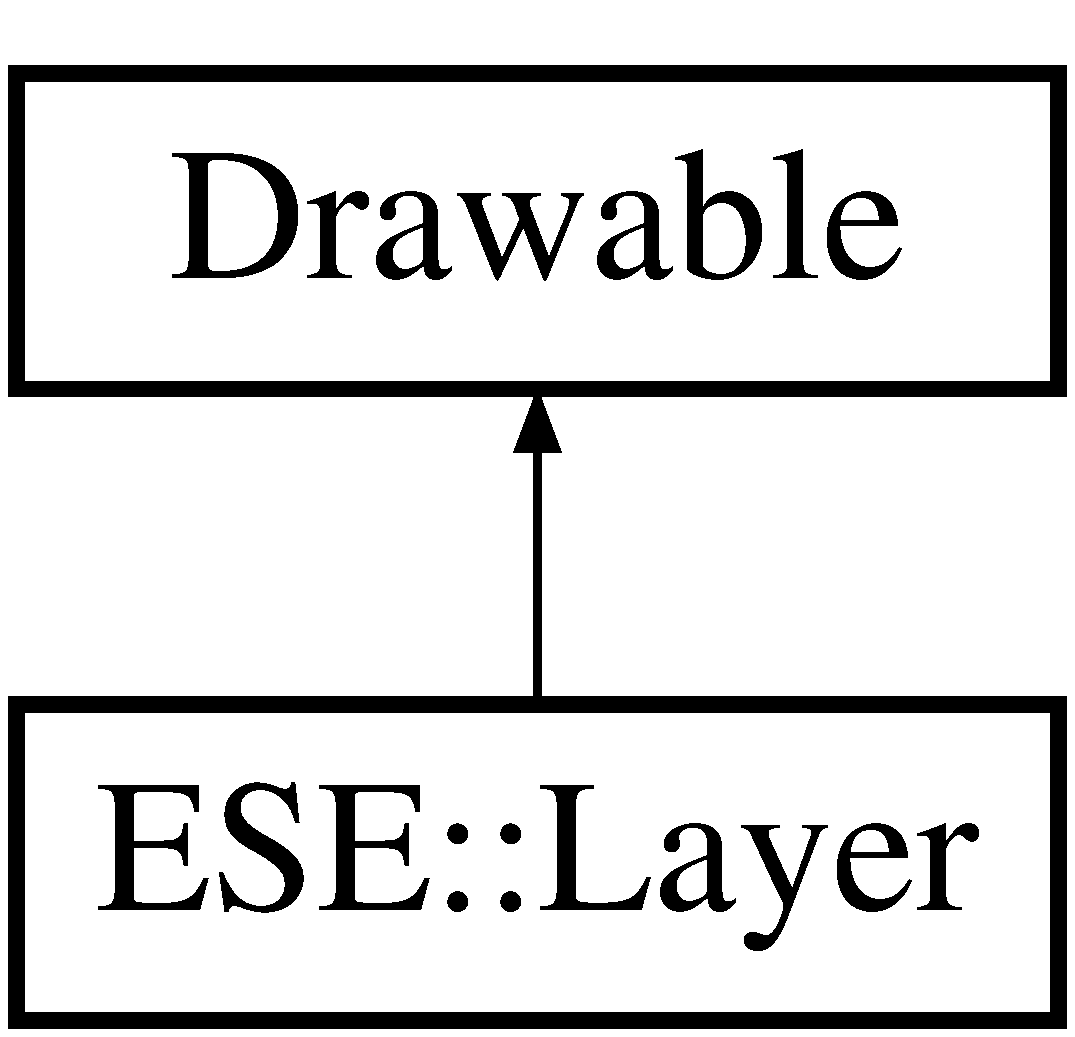
\includegraphics[height=2.000000cm]{class_e_s_e_1_1_layer}
\end{center}
\end{figure}
\subsection*{Métodos públicos}
\begin{DoxyCompactItemize}
\item 
\hypertarget{class_e_s_e_1_1_layer_a29459f6e01ded4118f92d69b8d4e18b8}{virtual void {\bfseries draw} (sf\-::\-Render\-Target \&target, sf\-::\-Render\-States states) const }\label{class_e_s_e_1_1_layer_a29459f6e01ded4118f92d69b8d4e18b8}

\item 
\hypertarget{class_e_s_e_1_1_layer_a46f97adf22072271198b24002bcab4f6}{void {\bfseries add\-Drawable} (sf\-::\-Drawable $\ast$item)}\label{class_e_s_e_1_1_layer_a46f97adf22072271198b24002bcab4f6}

\item 
\hypertarget{class_e_s_e_1_1_layer_a0fbd403cb05959adb7d9d2e84d37ec52}{void {\bfseries set\-Visible} (bool visible)}\label{class_e_s_e_1_1_layer_a0fbd403cb05959adb7d9d2e84d37ec52}

\end{DoxyCompactItemize}
\subsection*{Atributos protegidos}
\begin{DoxyCompactItemize}
\item 
\hypertarget{class_e_s_e_1_1_layer_aa1a201122fc3764662cc990b948c8093}{bool {\bfseries visible}}\label{class_e_s_e_1_1_layer_aa1a201122fc3764662cc990b948c8093}

\item 
\hypertarget{class_e_s_e_1_1_layer_a354d1f6a45375d8fce644f6c218a6127}{std\-::vector$<$ sf\-::\-Drawable $\ast$ $>$ {\bfseries drawable\-Items}}\label{class_e_s_e_1_1_layer_a354d1f6a45375d8fce644f6c218a6127}

\end{DoxyCompactItemize}


La documentación para esta clase fue generada a partir de los siguientes ficheros\-:\begin{DoxyCompactItemize}
\item 
include/\-E\-S\-E/\-Core/Layer.\-hpp\item 
src/\-E\-S\-E/\-Core/Layer.\-cpp\end{DoxyCompactItemize}

\hypertarget{class_e_s_e_1_1_log}{\section{Referencia de la Clase E\-S\-E\-:\-:Log}
\label{class_e_s_e_1_1_log}\index{E\-S\-E\-::\-Log@{E\-S\-E\-::\-Log}}
}
\subsection*{Tipos públicos}
\begin{DoxyCompactItemize}
\item 
enum \{ {\bfseries K\-E\-E\-P\-\_\-\-P\-R\-E\-V\-I\-O\-U\-S\-\_\-\-L\-O\-G}, 
{\bfseries R\-E\-M\-O\-V\-E\-\_\-\-P\-R\-E\-V\-I\-O\-U\-S\-\_\-\-L\-O\-G}
 \}
\end{DoxyCompactItemize}
\subsection*{Métodos públicos estáticos}
\begin{DoxyCompactItemize}
\item 
static bool \hyperlink{class_e_s_e_1_1_log_a1c99ca7fcbbe1dc7c3452a23c424e702}{open} (int mode=K\-E\-E\-P\-\_\-\-P\-R\-E\-V\-I\-O\-U\-S\-\_\-\-L\-O\-G)
\begin{DoxyCompactList}\small\item\em Abre el archivo de log para ser escrito. \end{DoxyCompactList}\item 
\hypertarget{class_e_s_e_1_1_log_a604725d638e15ebc07d67b433671d9ae}{static void \hyperlink{class_e_s_e_1_1_log_a604725d638e15ebc07d67b433671d9ae}{close} ()}\label{class_e_s_e_1_1_log_a604725d638e15ebc07d67b433671d9ae}

\begin{DoxyCompactList}\small\item\em Cierra el archivo, no se podrá escribir en él después de liberarlo. \end{DoxyCompactList}\item 
static void \hyperlink{class_e_s_e_1_1_log_a9383493aa4fe986699af44f933ae0b1b}{post} (std\-::string tag, std\-::string message)
\begin{DoxyCompactList}\small\item\em Escribe una entrada en el archivo de log. \end{DoxyCompactList}\item 
static void \hyperlink{class_e_s_e_1_1_log_a7a97f99bd8fb2425cf82641c470f2914}{error} (std\-::string message)
\begin{DoxyCompactList}\small\item\em Escribe una entrada con el tag E\-R\-R (error). \end{DoxyCompactList}\item 
static void \hyperlink{class_e_s_e_1_1_log_abbd0b1b08fc6dc5a331a402b25aa3c01}{warning} (std\-::string message)
\begin{DoxyCompactList}\small\item\em Escribe una entrada con el tag W\-A\-R (warning). \end{DoxyCompactList}\item 
static void \hyperlink{class_e_s_e_1_1_log_a06a6956c153b3add127b76b4a9fa86c2}{information} (std\-::string message)
\begin{DoxyCompactList}\small\item\em Escribe una entrada con el tag I\-N\-F (información). \end{DoxyCompactList}\end{DoxyCompactItemize}


\subsection{Documentación de las funciones miembro}
\hypertarget{class_e_s_e_1_1_log_a7a97f99bd8fb2425cf82641c470f2914}{\index{E\-S\-E\-::\-Log@{E\-S\-E\-::\-Log}!error@{error}}
\index{error@{error}!ESE::Log@{E\-S\-E\-::\-Log}}
\subsubsection[{error}]{\setlength{\rightskip}{0pt plus 5cm}void E\-S\-E\-::\-Log\-::error (
\begin{DoxyParamCaption}
\item[{std\-::string}]{message}
\end{DoxyParamCaption}
)\hspace{0.3cm}{\ttfamily [static]}}}\label{class_e_s_e_1_1_log_a7a97f99bd8fb2425cf82641c470f2914}


Escribe una entrada con el tag E\-R\-R (error). 


\begin{DoxyParams}{Parámetros}
{\em message} & Mensaje de error. Este método hace uso de \hyperlink{class_e_s_e_1_1_log_a9383493aa4fe986699af44f933ae0b1b}{post()} al que envía como etiqueta \char`\"{}\-E\-R\-R\char`\"{}. \\
\hline
\end{DoxyParams}
\hypertarget{class_e_s_e_1_1_log_a06a6956c153b3add127b76b4a9fa86c2}{\index{E\-S\-E\-::\-Log@{E\-S\-E\-::\-Log}!information@{information}}
\index{information@{information}!ESE::Log@{E\-S\-E\-::\-Log}}
\subsubsection[{information}]{\setlength{\rightskip}{0pt plus 5cm}void E\-S\-E\-::\-Log\-::information (
\begin{DoxyParamCaption}
\item[{std\-::string}]{message}
\end{DoxyParamCaption}
)\hspace{0.3cm}{\ttfamily [static]}}}\label{class_e_s_e_1_1_log_a06a6956c153b3add127b76b4a9fa86c2}


Escribe una entrada con el tag I\-N\-F (información). 


\begin{DoxyParams}{Parámetros}
{\em message} & Mensaje informativo. Este método hace uso de \hyperlink{class_e_s_e_1_1_log_a9383493aa4fe986699af44f933ae0b1b}{post()} al que envía como etiqueta \char`\"{}\-I\-N\-F\char`\"{}. \\
\hline
\end{DoxyParams}
\hypertarget{class_e_s_e_1_1_log_a1c99ca7fcbbe1dc7c3452a23c424e702}{\index{E\-S\-E\-::\-Log@{E\-S\-E\-::\-Log}!open@{open}}
\index{open@{open}!ESE::Log@{E\-S\-E\-::\-Log}}
\subsubsection[{open}]{\setlength{\rightskip}{0pt plus 5cm}bool E\-S\-E\-::\-Log\-::open (
\begin{DoxyParamCaption}
\item[{int}]{mode = {\ttfamily KEEP\-\_\-PREVIOUS\-\_\-LOG}}
\end{DoxyParamCaption}
)\hspace{0.3cm}{\ttfamily [static]}}}\label{class_e_s_e_1_1_log_a1c99ca7fcbbe1dc7c3452a23c424e702}


Abre el archivo de log para ser escrito. 


\begin{DoxyParams}{Parámetros}
{\em M\-O\-D\-E} & Modo de apertura. Si es K\-E\-E\-P\-\_\-\-P\-R\-E\-V\-I\-O\-U\-S\-\_\-\-L\-O\-G no se perderá el log anterior. Si es R\-E\-M\-O\-V\-E\-\_\-\-P\-R\-E\-V\-I\-O\-U\-S\-\_\-\-L\-O\-G se sobreescribirá. \\
\hline
\end{DoxyParams}
\begin{DoxyReturn}{Devuelve}
T\-R\-U\-E si el archivo está abierto y se puede escribir, si no, F\-A\-L\-S\-E. 
\end{DoxyReturn}
\hypertarget{class_e_s_e_1_1_log_a9383493aa4fe986699af44f933ae0b1b}{\index{E\-S\-E\-::\-Log@{E\-S\-E\-::\-Log}!post@{post}}
\index{post@{post}!ESE::Log@{E\-S\-E\-::\-Log}}
\subsubsection[{post}]{\setlength{\rightskip}{0pt plus 5cm}void E\-S\-E\-::\-Log\-::post (
\begin{DoxyParamCaption}
\item[{std\-::string}]{tag, }
\item[{std\-::string}]{message}
\end{DoxyParamCaption}
)\hspace{0.3cm}{\ttfamily [static]}}}\label{class_e_s_e_1_1_log_a9383493aa4fe986699af44f933ae0b1b}


Escribe una entrada en el archivo de log. 


\begin{DoxyParams}{Parámetros}
{\em tag} & La etiqueta que tendrá el mensaje. \\
\hline
{\em message} & El mensaje que queremos escribir después de la etiqueta. Cuando llamamos a esta función, escribiremos una línea en el archivo de así\-:\par
 T\-A\-G M\-E\-N\-S\-A\-J\-E Entre ambos hay una tabulación. \\
\hline
\end{DoxyParams}
\hypertarget{class_e_s_e_1_1_log_abbd0b1b08fc6dc5a331a402b25aa3c01}{\index{E\-S\-E\-::\-Log@{E\-S\-E\-::\-Log}!warning@{warning}}
\index{warning@{warning}!ESE::Log@{E\-S\-E\-::\-Log}}
\subsubsection[{warning}]{\setlength{\rightskip}{0pt plus 5cm}void E\-S\-E\-::\-Log\-::warning (
\begin{DoxyParamCaption}
\item[{std\-::string}]{message}
\end{DoxyParamCaption}
)\hspace{0.3cm}{\ttfamily [static]}}}\label{class_e_s_e_1_1_log_abbd0b1b08fc6dc5a331a402b25aa3c01}


Escribe una entrada con el tag W\-A\-R (warning). 


\begin{DoxyParams}{Parámetros}
{\em message} & Mensaje de warning. Este método hace uso de \hyperlink{class_e_s_e_1_1_log_a9383493aa4fe986699af44f933ae0b1b}{post()} al que envía como etiqueta \char`\"{}\-W\-A\-R\char`\"{}. \\
\hline
\end{DoxyParams}


La documentación para esta clase fue generada a partir de los siguientes ficheros\-:\begin{DoxyCompactItemize}
\item 
include/\-E\-S\-E/\-Core/Log.\-hpp\item 
src/\-E\-S\-E/\-Core/Log.\-cpp\end{DoxyCompactItemize}

\hypertarget{class_e_s_e_1_1_resource_container}{\section{Referencia de la plantilla de la Clase E\-S\-E\-:\-:Resource\-Container$<$ T $>$}
\label{class_e_s_e_1_1_resource_container}\index{E\-S\-E\-::\-Resource\-Container$<$ T $>$@{E\-S\-E\-::\-Resource\-Container$<$ T $>$}}
}
\subsection*{Métodos públicos}
\begin{DoxyCompactItemize}
\item 
\hypertarget{class_e_s_e_1_1_resource_container_aaa52f82fc184b161ef4dc79f4c23b456}{virtual T $\ast$ {\bfseries get\-Resource} (std\-::string name, bool test\-If\-Exists=true)}\label{class_e_s_e_1_1_resource_container_aaa52f82fc184b161ef4dc79f4c23b456}

\end{DoxyCompactItemize}
\subsection*{Métodos protegidos}
\begin{DoxyCompactItemize}
\item 
\hypertarget{class_e_s_e_1_1_resource_container_a5a42af790f1a6baec2b426b20ab65989}{virtual void {\bfseries load\-From\-File} (std\-::string name, std\-::string path)=0}\label{class_e_s_e_1_1_resource_container_a5a42af790f1a6baec2b426b20ab65989}

\end{DoxyCompactItemize}
\subsection*{Atributos protegidos}
\begin{DoxyCompactItemize}
\item 
\hypertarget{class_e_s_e_1_1_resource_container_a520346f25f7e73e23751e1b2758784ab}{std\-::map$<$ std\-::string, T $>$ {\bfseries resources}}\label{class_e_s_e_1_1_resource_container_a520346f25f7e73e23751e1b2758784ab}

\end{DoxyCompactItemize}


La documentación para esta clase fue generada a partir del siguiente fichero\-:\begin{DoxyCompactItemize}
\item 
include/\-E\-S\-E/\-Core/Resource\-Container.\-hpp\end{DoxyCompactItemize}

\hypertarget{class_e_s_e_1_1_resource_manager}{\section{Referencia de la Clase E\-S\-E\-:\-:Resource\-Manager}
\label{class_e_s_e_1_1_resource_manager}\index{E\-S\-E\-::\-Resource\-Manager@{E\-S\-E\-::\-Resource\-Manager}}
}
\subsection*{Métodos públicos}
\begin{DoxyCompactItemize}
\item 
\hypertarget{class_e_s_e_1_1_resource_manager_a6e85562647c3019c6fc962da20b19b39}{\hyperlink{class_e_s_e_1_1_texture_container}{E\-S\-E\-::\-Texture\-Container} $\ast$ {\bfseries get\-Texture\-Container} ()}\label{class_e_s_e_1_1_resource_manager_a6e85562647c3019c6fc962da20b19b39}

\end{DoxyCompactItemize}
\subsection*{Métodos públicos estáticos}
\begin{DoxyCompactItemize}
\item 
\hypertarget{class_e_s_e_1_1_resource_manager_ac4ef3febefc36ede251ea774a6c8450e}{static \hyperlink{class_e_s_e_1_1_resource_manager}{Resource\-Manager} $\ast$ {\bfseries instance} ()}\label{class_e_s_e_1_1_resource_manager_ac4ef3febefc36ede251ea774a6c8450e}

\item 
\hypertarget{class_e_s_e_1_1_resource_manager_a9bfdec5aa68922972490c313d38d9f80}{static void {\bfseries release} ()}\label{class_e_s_e_1_1_resource_manager_a9bfdec5aa68922972490c313d38d9f80}

\end{DoxyCompactItemize}
\subsection*{Atributos protegidos}
\begin{DoxyCompactItemize}
\item 
\hypertarget{class_e_s_e_1_1_resource_manager_a9c461d4def6d321a968fc6a230341222}{\hyperlink{class_e_s_e_1_1_texture_container}{E\-S\-E\-::\-Texture\-Container} {\bfseries texture\-Container}}\label{class_e_s_e_1_1_resource_manager_a9c461d4def6d321a968fc6a230341222}

\end{DoxyCompactItemize}


La documentación para esta clase fue generada a partir de los siguientes ficheros\-:\begin{DoxyCompactItemize}
\item 
include/\-E\-S\-E/\-Core/Resource\-Manager.\-hpp\item 
src/\-E\-S\-E/\-Core/Resource\-Manager.\-cpp\end{DoxyCompactItemize}

\hypertarget{class_e_s_e_1_1_scene}{\section{Referencia de la Clase E\-S\-E\-:\-:Scene}
\label{class_e_s_e_1_1_scene}\index{E\-S\-E\-::\-Scene@{E\-S\-E\-::\-Scene}}
}
\subsection*{Tipos públicos}
\begin{DoxyCompactItemize}
\item 
enum {\bfseries State} \{ {\bfseries Active}, 
{\bfseries Background}, 
{\bfseries Inactive}
 \}
\end{DoxyCompactItemize}
\subsection*{Métodos públicos}
\begin{DoxyCompactItemize}
\item 
\hypertarget{class_e_s_e_1_1_scene_a93bf19aa1d39de6681720062849424ec}{{\bfseries Scene} (sf\-::\-Render\-Window $\ast$window)}\label{class_e_s_e_1_1_scene_a93bf19aa1d39de6681720062849424ec}

\item 
\hypertarget{class_e_s_e_1_1_scene_abdb55959ba27e7bef73ab2cc4cb14bb9}{virtual State {\bfseries get\-State} ()}\label{class_e_s_e_1_1_scene_abdb55959ba27e7bef73ab2cc4cb14bb9}

\item 
\hypertarget{class_e_s_e_1_1_scene_ac4c38efa12cce119b3553a4e07c1db88}{virtual void {\bfseries set\-Window} (sf\-::\-Render\-Window $\ast$window)}\label{class_e_s_e_1_1_scene_ac4c38efa12cce119b3553a4e07c1db88}

\end{DoxyCompactItemize}
\subsection*{Métodos protegidos}
\begin{DoxyCompactItemize}
\item 
\hypertarget{class_e_s_e_1_1_scene_a22866cba7abec763ea9ae911a21413b5}{virtual void {\bfseries start} ()}\label{class_e_s_e_1_1_scene_a22866cba7abec763ea9ae911a21413b5}

\item 
\hypertarget{class_e_s_e_1_1_scene_a1c960d5be844bf7b9855a52e9ca387b3}{virtual void {\bfseries stop} ()}\label{class_e_s_e_1_1_scene_a1c960d5be844bf7b9855a52e9ca387b3}

\item 
\hypertarget{class_e_s_e_1_1_scene_a6bd8bc1dc787f5ce8bcdf87680d54882}{virtual void {\bfseries pause} ()}\label{class_e_s_e_1_1_scene_a6bd8bc1dc787f5ce8bcdf87680d54882}

\item 
\hypertarget{class_e_s_e_1_1_scene_a72a3225383964d3e947017fa6cd4fff7}{virtual void {\bfseries set\-State} (State state)}\label{class_e_s_e_1_1_scene_a72a3225383964d3e947017fa6cd4fff7}

\item 
\hypertarget{class_e_s_e_1_1_scene_a83f9a4b9ee1b1a398bec564689fb8aa6}{virtual void {\bfseries gameloop} (float delta\-Time)}\label{class_e_s_e_1_1_scene_a83f9a4b9ee1b1a398bec564689fb8aa6}

\item 
\hypertarget{class_e_s_e_1_1_scene_a4d76f82cec698eb2b75cd3de3510a84c}{virtual void {\bfseries manage\-Events} ()}\label{class_e_s_e_1_1_scene_a4d76f82cec698eb2b75cd3de3510a84c}

\item 
\hypertarget{class_e_s_e_1_1_scene_a45d89e1c2e1b52b056539ddad9941540}{virtual void {\bfseries logic} ()}\label{class_e_s_e_1_1_scene_a45d89e1c2e1b52b056539ddad9941540}

\item 
\hypertarget{class_e_s_e_1_1_scene_ae023ad47de46ea1f5cda35ee3347eb37}{virtual void {\bfseries render} ()}\label{class_e_s_e_1_1_scene_ae023ad47de46ea1f5cda35ee3347eb37}

\item 
\hypertarget{class_e_s_e_1_1_scene_af97af9f21553e082e9bdb65067acd3e8}{virtual void {\bfseries check\-If\-Window\-Closed} ()}\label{class_e_s_e_1_1_scene_af97af9f21553e082e9bdb65067acd3e8}

\end{DoxyCompactItemize}
\subsection*{Atributos protegidos}
\begin{DoxyCompactItemize}
\item 
\hypertarget{class_e_s_e_1_1_scene_a0d460f2365daaf835c7f36cbce28cd42}{State {\bfseries state}}\label{class_e_s_e_1_1_scene_a0d460f2365daaf835c7f36cbce28cd42}

\item 
\hypertarget{class_e_s_e_1_1_scene_aeba78c8125ff759da93cfeadf89bf1f2}{sf\-::\-Render\-Window $\ast$ {\bfseries window}}\label{class_e_s_e_1_1_scene_aeba78c8125ff759da93cfeadf89bf1f2}

\item 
\hypertarget{class_e_s_e_1_1_scene_a2086a9c827c7cc684d7e36a757d5ff3b}{sf\-::\-Event {\bfseries events}}\label{class_e_s_e_1_1_scene_a2086a9c827c7cc684d7e36a757d5ff3b}

\end{DoxyCompactItemize}
\subsection*{Amigas}
\begin{DoxyCompactItemize}
\item 
\hypertarget{class_e_s_e_1_1_scene_a284464b0561a6f2915f04b0245b987f0}{class {\bfseries Scene\-Manager}}\label{class_e_s_e_1_1_scene_a284464b0561a6f2915f04b0245b987f0}

\end{DoxyCompactItemize}


La documentación para esta clase fue generada a partir de los siguientes ficheros\-:\begin{DoxyCompactItemize}
\item 
include/\-E\-S\-E/\-Core/Scene.\-hpp\item 
src/\-E\-S\-E/\-Core/Scene.\-cpp\end{DoxyCompactItemize}

\hypertarget{class_e_s_e_1_1_scene_manager}{\section{Referencia de la Clase E\-S\-E\-:\-:Scene\-Manager}
\label{class_e_s_e_1_1_scene_manager}\index{E\-S\-E\-::\-Scene\-Manager@{E\-S\-E\-::\-Scene\-Manager}}
}
\subsection*{Métodos públicos}
\begin{DoxyCompactItemize}
\item 
\hypertarget{class_e_s_e_1_1_scene_manager_a8e015c62baeba7ec62bf52494b977cf9}{void {\bfseries add\-Scene} (std\-::string name, \hyperlink{class_e_s_e_1_1_scene}{E\-S\-E\-::\-Scene} $\ast$scene, bool dont\-Add\-If\-Exists=false)}\label{class_e_s_e_1_1_scene_manager_a8e015c62baeba7ec62bf52494b977cf9}

\item 
void \hyperlink{class_e_s_e_1_1_scene_manager_a8604839d539ecf138d3b773679d64396}{manage} ()
\item 
\hypertarget{class_e_s_e_1_1_scene_manager_af726a9763ab3f9fec3ed87c7e5859f3f}{void {\bfseries activate\-Scene} (std\-::string name)}\label{class_e_s_e_1_1_scene_manager_af726a9763ab3f9fec3ed87c7e5859f3f}

\item 
\hypertarget{class_e_s_e_1_1_scene_manager_ac35af6a5448740a9038f33e17bacb514}{void {\bfseries activate\-Scene\-And\-Deactivate\-The\-Rest} (std\-::string name)}\label{class_e_s_e_1_1_scene_manager_ac35af6a5448740a9038f33e17bacb514}

\item 
\hypertarget{class_e_s_e_1_1_scene_manager_ad2dc75bba3b9e480510228cd0288377e}{void {\bfseries deactivate\-Scene} (std\-::string name)}\label{class_e_s_e_1_1_scene_manager_ad2dc75bba3b9e480510228cd0288377e}

\item 
\hypertarget{class_e_s_e_1_1_scene_manager_a47a2b80f898c24a013b88bf27e941de0}{void {\bfseries deactivate\-All\-Scenes} ()}\label{class_e_s_e_1_1_scene_manager_a47a2b80f898c24a013b88bf27e941de0}

\item 
\hypertarget{class_e_s_e_1_1_scene_manager_ad7ccd504949840f0b128d86e519fe11d}{void {\bfseries sent\-Scene\-To\-Background} (std\-::string name)}\label{class_e_s_e_1_1_scene_manager_ad7ccd504949840f0b128d86e519fe11d}

\end{DoxyCompactItemize}
\subsection*{Métodos públicos estáticos}
\begin{DoxyCompactItemize}
\item 
\hypertarget{class_e_s_e_1_1_scene_manager_aaaa89971bb80990b3a81373288611707}{static \hyperlink{class_e_s_e_1_1_scene_manager}{Scene\-Manager} $\ast$ {\bfseries instance} (sf\-::\-Render\-Window $\ast$window=N\-U\-L\-L)}\label{class_e_s_e_1_1_scene_manager_aaaa89971bb80990b3a81373288611707}

\item 
\hypertarget{class_e_s_e_1_1_scene_manager_a5b0684cc0813e996c76b99bee1bb2afc}{static void {\bfseries release} ()}\label{class_e_s_e_1_1_scene_manager_a5b0684cc0813e996c76b99bee1bb2afc}

\end{DoxyCompactItemize}
\subsection*{Métodos protegidos}
\begin{DoxyCompactItemize}
\item 
\hypertarget{class_e_s_e_1_1_scene_manager_a6d218fbaf082f65d8ed1a0160e39b0e2}{void {\bfseries start\-Render} ()}\label{class_e_s_e_1_1_scene_manager_a6d218fbaf082f65d8ed1a0160e39b0e2}

\item 
\hypertarget{class_e_s_e_1_1_scene_manager_aad06a2b77464393deb4aa5fb2814529d}{void {\bfseries stop\-Render} ()}\label{class_e_s_e_1_1_scene_manager_aad06a2b77464393deb4aa5fb2814529d}

\item 
\hypertarget{class_e_s_e_1_1_scene_manager_a567e482476f30f59ddd1558985cea345}{\hyperlink{class_e_s_e_1_1_scene}{Scene} $\ast$ {\bfseries look\-For\-Scene} (std\-::string nombre)}\label{class_e_s_e_1_1_scene_manager_a567e482476f30f59ddd1558985cea345}

\end{DoxyCompactItemize}
\subsection*{Atributos protegidos}
\begin{DoxyCompactItemize}
\item 
\hypertarget{class_e_s_e_1_1_scene_manager_a5923c00d505856472745e7e0d4aa0039}{sf\-::\-Render\-Window $\ast$ {\bfseries window}}\label{class_e_s_e_1_1_scene_manager_a5923c00d505856472745e7e0d4aa0039}

\item 
\hypertarget{class_e_s_e_1_1_scene_manager_a43d2a66fcf59d4718cabc7091ad73048}{std\-::vector$<$ std\-::pair\\*
$<$ std\-::string, \hyperlink{class_e_s_e_1_1_scene}{E\-S\-E\-::\-Scene} $\ast$ $>$ $>$ {\bfseries scenes}}\label{class_e_s_e_1_1_scene_manager_a43d2a66fcf59d4718cabc7091ad73048}

\item 
\hypertarget{class_e_s_e_1_1_scene_manager_a24372f1d7bd11a221f9b6bacad7b892d}{sf\-::\-Clock {\bfseries delta\-Time}}\label{class_e_s_e_1_1_scene_manager_a24372f1d7bd11a221f9b6bacad7b892d}

\end{DoxyCompactItemize}
\subsection*{Atributos protegidos estáticos}
\begin{DoxyCompactItemize}
\item 
\hypertarget{class_e_s_e_1_1_scene_manager_aa7919de1717ea80294ed72286047e472}{static \hyperlink{class_e_s_e_1_1_scene_manager}{Scene\-Manager} $\ast$ {\bfseries scene\-Manager\-Instance} = 0}\label{class_e_s_e_1_1_scene_manager_aa7919de1717ea80294ed72286047e472}

\end{DoxyCompactItemize}


\subsection{Documentación de las funciones miembro}
\hypertarget{class_e_s_e_1_1_scene_manager_a8604839d539ecf138d3b773679d64396}{\index{E\-S\-E\-::\-Scene\-Manager@{E\-S\-E\-::\-Scene\-Manager}!manage@{manage}}
\index{manage@{manage}!ESE::SceneManager@{E\-S\-E\-::\-Scene\-Manager}}
\subsubsection[{manage}]{\setlength{\rightskip}{0pt plus 5cm}void E\-S\-E\-::\-Scene\-Manager\-::manage (
\begin{DoxyParamCaption}
{}
\end{DoxyParamCaption}
)}}\label{class_e_s_e_1_1_scene_manager_a8604839d539ecf138d3b773679d64396}
Si no hay ninguna activa, salimos del bucle. 

La documentación para esta clase fue generada a partir de los siguientes ficheros\-:\begin{DoxyCompactItemize}
\item 
include/\-E\-S\-E/\-Core/Scene\-Manager.\-hpp\item 
src/\-E\-S\-E/\-Core/Scene\-Manager.\-cpp\end{DoxyCompactItemize}

\hypertarget{class_e_s_e_1_1_text}{\section{Referencia de la Clase E\-S\-E\-:\-:Text}
\label{class_e_s_e_1_1_text}\index{E\-S\-E\-::\-Text@{E\-S\-E\-::\-Text}}
}
\subsection*{Métodos públicos}
\begin{DoxyCompactItemize}
\item 
\hypertarget{class_e_s_e_1_1_text_a5d3237d7ab89c455431bb0f4a5f9eeaf}{{\bfseries Text} (std\-::string file, std\-::string language)}\label{class_e_s_e_1_1_text_a5d3237d7ab89c455431bb0f4a5f9eeaf}

\item 
\hypertarget{class_e_s_e_1_1_text_a2675ac2e591125b1596fd974690f1959}{void {\bfseries load} (std\-::string file, std\-::string language)}\label{class_e_s_e_1_1_text_a2675ac2e591125b1596fd974690f1959}

\item 
\hypertarget{class_e_s_e_1_1_text_ab6d418629ec56847f887d15de644d382}{std\-::string {\bfseries get\-String} (std\-::string name)}\label{class_e_s_e_1_1_text_ab6d418629ec56847f887d15de644d382}

\item 
\hypertarget{class_e_s_e_1_1_text_ae30f8644d8994d366005f97ca6a73922}{std\-::string {\bfseries get\-Current\-Language} ()}\label{class_e_s_e_1_1_text_ae30f8644d8994d366005f97ca6a73922}

\end{DoxyCompactItemize}
\subsection*{Atributos protegidos}
\begin{DoxyCompactItemize}
\item 
\hypertarget{class_e_s_e_1_1_text_a4ac577bffe650d9a49f5793f52e04a8d}{std\-::map$<$ std\-::string, \\*
std\-::string $>$ {\bfseries content}}\label{class_e_s_e_1_1_text_a4ac577bffe650d9a49f5793f52e04a8d}

\item 
\hypertarget{class_e_s_e_1_1_text_ac108b56c1a1e7b49b1c14c5a9076782e}{std\-::string {\bfseries current\-Language}}\label{class_e_s_e_1_1_text_ac108b56c1a1e7b49b1c14c5a9076782e}

\end{DoxyCompactItemize}


La documentación para esta clase fue generada a partir de los siguientes ficheros\-:\begin{DoxyCompactItemize}
\item 
include/\-E\-S\-E/\-Text/Text.\-hpp\item 
src/\-E\-S\-E/\-Text/Text.\-cpp\end{DoxyCompactItemize}

\hypertarget{class_e_s_e_1_1_texture_container}{\section{Referencia de la Clase E\-S\-E\-:\-:Texture\-Container}
\label{class_e_s_e_1_1_texture_container}\index{E\-S\-E\-::\-Texture\-Container@{E\-S\-E\-::\-Texture\-Container}}
}
Diagrama de herencias de E\-S\-E\-:\-:Texture\-Container\begin{figure}[H]
\begin{center}
\leavevmode
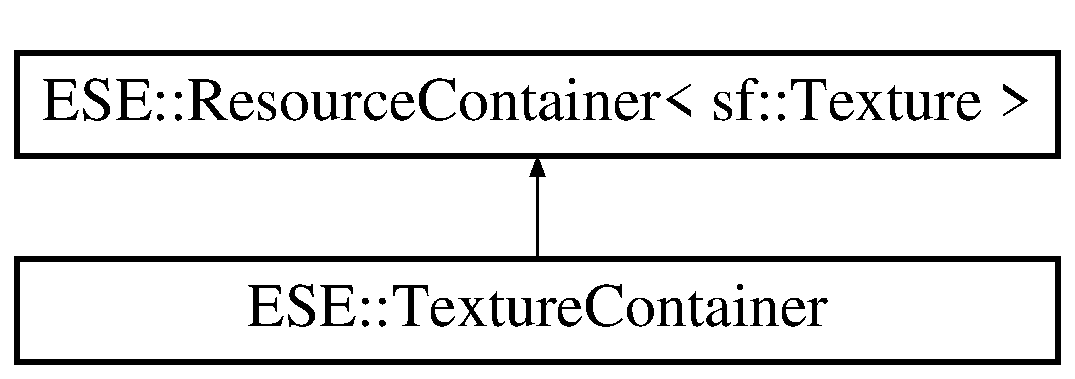
\includegraphics[height=2.000000cm]{class_e_s_e_1_1_texture_container}
\end{center}
\end{figure}
\subsection*{Métodos públicos}
\begin{DoxyCompactItemize}
\item 
\hypertarget{class_e_s_e_1_1_texture_container_a942ccb0fc6d4f59b58552e61cf366b55}{virtual void {\bfseries load\-From\-File} (std\-::string name, std\-::string path)}\label{class_e_s_e_1_1_texture_container_a942ccb0fc6d4f59b58552e61cf366b55}

\end{DoxyCompactItemize}
\subsection*{Otros miembros heredados}


La documentación para esta clase fue generada a partir de los siguientes ficheros\-:\begin{DoxyCompactItemize}
\item 
include/\-E\-S\-E/\-Core/Texture\-Container.\-hpp\item 
src/\-E\-S\-E/\-Core/Texture\-Container.\-cpp\end{DoxyCompactItemize}

%--- End generated contents ---

% Index
\newpage
\phantomsection
\addcontentsline{toc}{chapter}{Índice}
\printindex

\end{document}
